\documentclass[mathserif,serif]{beamer}
\usetheme{Warsaw}
\usepackage[utf8]{inputenc}
\usepackage[russian]{babel}
\usepackage{listings}

\title[Безопасное хранение секретов]
{Безопасное хранение секретов}
\subtitle{Опыт использования Hashicorp Vault}
\date
{}

\begin{document}
\frame{\titlepage}

\begin{frame}
	\frametitle{Безопасность - всему голова}
	
\includegraphics[width=\linewidth]{sieve.jpg}
\end{frame}

\begin{frame}
	\frametitle{Ключи непосредственно на машинах}
	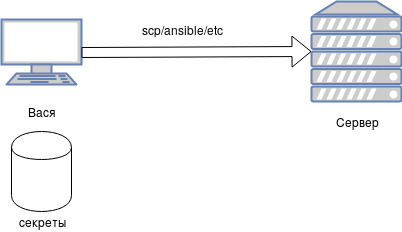
\includegraphics[width=\linewidth]{primitive1.png}
\end{frame}

\begin{frame}
	\frametitle{Ключи в репозитории}
	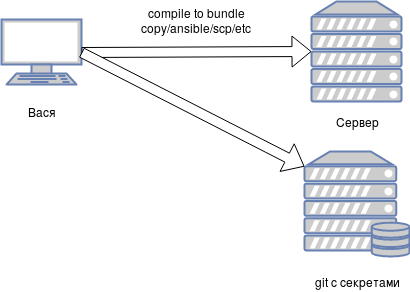
\includegraphics[width=\linewidth]{primitive2.png}
\end{frame}

\begin{frame}
	\frametitle{И что с того?}
	\begin{itemize}
		\item{Человеческий фактор}
		\item{Неудобство использования}
		\item{Потенциальная уязвимость секретов}
	\end{itemize}
\end{frame}

\begin{frame}
	\frametitle{Давным-давно, при динозаврах}
	
\includegraphics[width=\linewidth]{dino.jpg}
\end{frame}

\begin{frame}
	\frametitle{Hashicorp Vault}
	\begin{itemize}
		\item{Безопасное и надежное хранение}
		\item{Обновление секретов}
		\item{Аудит использования}
		\item{Генерация используя бэкенды}
		\item{Система плагинов}
	\end{itemize}
\end{frame}

\begin{frame}
	\frametitle{Хранилища}
	\begin{itemize}
		\item{Azure}
		\item{Consul}
		\item{Etcd}
		\item{In-Memory}
		\item{MySQL}
		\item{Zookeeper}
		\item{другие}
	\end{itemize}
\end{frame}

\begin{frame}
	\frametitle{Consul storage}
	\begin{itemize}
		\item{Регистрация в консуле из коробки}
		\item{Высокая доступность}
		\item{Данные в консуле в зашифрованном виде}
		\item{Официальная поддержка}
		\item{У нас уже есть консул :)}
	\end{itemize}
\end{frame}

\begin{frame}
	\frametitle{Управление секретами используя бэкенд}
	\begin{itemize}
		\item{AWS}
		\item{Consul}
		\item{Mongo}
		\item{Postgres}
		\item{Nomad}
		\item{RabbitMQ}
		\item{другие}
	\end{itemize}
\end{frame}

\begin{frame}
	\frametitle{Авторизация в vault}
	\begin{itemize}
		\item{AWS EC2}
		\item{AWS IAM}
		\item{Tokens}
		\item{Kubernetes}
		\item{LDAP}
		\item{другие}
	\end{itemize}
\end{frame}

\begin{frame}
	\frametitle{AWS EC2}
	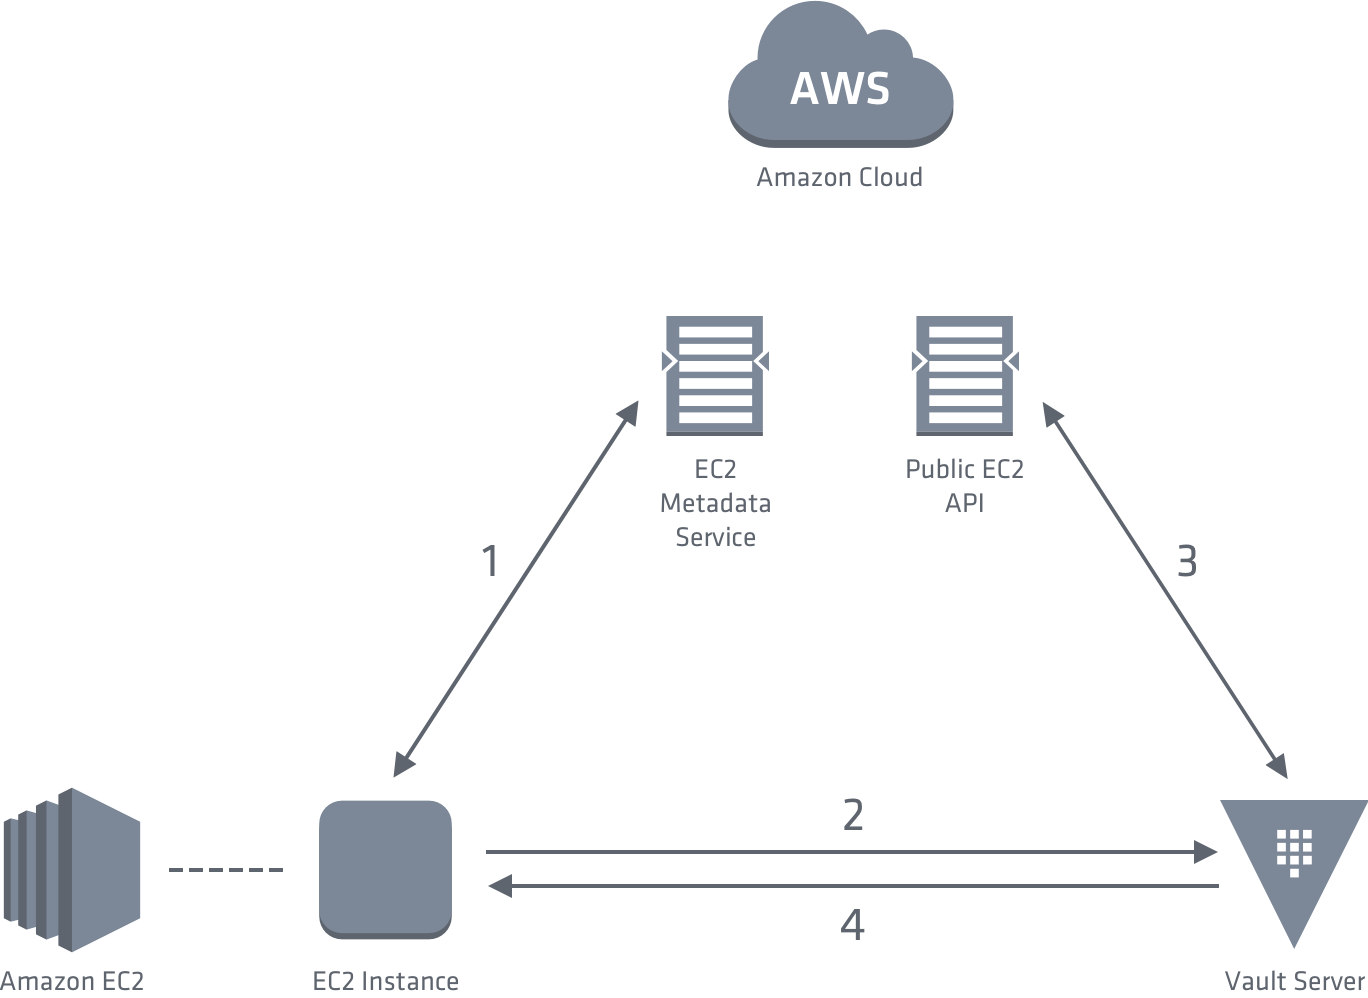
\includegraphics[width=0.8\linewidth]{ec2.png}
\end{frame}

\begin{frame}
	\frametitle{AWS EC2 - что происходит}
	\begin{itemize}
		\item{Получить подпись машины}
		\item{Запрос на токен с подписью отправляется в Vault}
		\item{Vault сверяет подпись машины через AWS API}
		\item{Vault token выдается в ответ на запрос}
		\item{Приложение использует токен для логина}
	\end{itemize}
\end{frame}

\begin{frame}
	\frametitle{Интересная часть}
	
\includegraphics[width=\linewidth]{gift.jpg}
\end{frame}

\begin{frame}
	\frametitle{Kubernetes - что такое}
	\begin{itemize}
		\item{Надежно хранимые ресурсы}
		\item{Контроллеры}
		\item{Да и всё}
	\end{itemize}
\end{frame}

\begin{frame}
	\frametitle{Kubernetes - ServiceAccount}
	\begin{itemize}
		\item{Биндинг политик доступа k8s}
		\item{Опциональный маунт k8s API токена (jwe)}
		\item{Доступ к секретам k8s}
	\end{itemize}
\end{frame}

\begin{frame}[fragile]
	\frametitle{Kubernetes - ServiceAccount - пример}
	\begin{verbatim}
apiVersion: v1
kind: ServiceAccount
metadata:
  name: myrestrictedaccount
  namespace: default
automountServiceAccountToken: true
	\end{verbatim}
\end{frame}

\begin{frame}[fragile]
	\frametitle{Kubernetes - джентельменский набор запуска}
	Приложения описываются ресурсом Pod
	\begin{verbatim}
apiVersion: v1
kind: Pod
metadata:
  name: app
spec:
  serviceAccountName: myrestrictedaccount
  containers:
    - name: app
      image: myapp:latest
	\end{verbatim}
\end{frame}

\begin{frame}
	\frametitle{Kubernetes + Vault}
	\begin{itemize}
		\item{Регистрируем кластер в Vault}
		\item{Ассоциируем ServiceAccount с ролью в Vault}
		\item{jwe API token k8s дает возможность выполнить логин}
	\end{itemize}
\end{frame}

\begin{frame}
	\frametitle{Terraform}
	\begin{itemize}
		\item{Infrastructure as code}
		\item{Инфраструктура как состояние}
		\item{Множество разных провайдеров}
	\end{itemize}
\end{frame}

\begin{frame}[fragile]
	\frametitle{Terraform + Kubernetes - Vault policy}
	\begin{verbatim}
resource "vault_policy" "example" {
  name = "some_policy"
  policy = <<EOT
path "secret/example" {
  policy = "read"
}
EOT
}
	\end{verbatim}
\end{frame}


\begin{frame}[fragile]
	\frametitle{Terraform + Kubernetes - Vault role}
	\begin{verbatim}
resource "vault_generic_secret" "vault_role" {
  path = "auth/kubernetes/role/vaultrolename"
  data_json = <<EOF
{
  "bound_service_account_names":      ["myrestrictedaccount"],
  "bound_service_account_namespaces": ["default"],
  "policies": ["some_policy"],
  "ttl": 3600
}EOF
}
	\end{verbatim}
\end{frame}

\begin{frame}[fragile]
	\frametitle{Kubernetes - SecretClaim}
	https://github.com/roboll/kube-vault-controller
	\begin{verbatim}
kind: SecretClaim
apiVersion: vaultproject.io/v1
metadata:
  name: some-secret
spec:
  type: Opaque
  path: secret/example
  renew: 3600
	\end{verbatim}
\end{frame}

\begin{frame}
	\frametitle{Резюме (не то что для найма)}
	\begin{itemize}
		\item{Vault решает задачи безопасного хранения секретов}
		\item{Тулинг работы с Vault и его интеграцией достаточно зрел}
		\item{Интеграция с Kubernetes доступна на разных уровнях}
		\item{В очередной раз спасибо Hashicorp}
	\end{itemize}
\end{frame}

\begin{frame}
	\frametitle{Вопросы?}
	
\includegraphics[width=\linewidth]{kitten.jpg}
\end{frame}

\end{document}